\documentclass[conference]{IEEEtran}
\IEEEoverridecommandlockouts

\usepackage{cite}
\usepackage{amsmath,amssymb,amsfonts}
\usepackage{algorithmic}
\usepackage[final]{graphicx}
\usepackage{textcomp}
\usepackage{xcolor}
\usepackage{booktabs}
\usepackage{array}
\usepackage{url}
\usepackage{hyperref}
\usepackage{float}
\usepackage{subcaption}
\usepackage{multirow}
\usepackage{siunitx}

\DeclareGraphicsExtensions{.png,.jpg,.pdf}

\hypersetup{
    colorlinks=true,
    linkcolor=blue,
    citecolor=blue,
    urlcolor=blue
}

\def\BibTeX{{\rm B\kern-.05em{\sc i\kern-.025em b}\kern-.08em
    T\kern-.1667em\lower.7ex\hbox{E}\kern-.125emX}}

\begin{document}

\title{%
  Adaptive Cyber-Physical Security:\\
  Semi-Supervised Anomaly-Based Intrusion Detection\\
  on the NSL-KDD Dataset
  \thanks{Phase 1 Baseline Report --- Advanced Machine Learning Project.}
}

\author{%
  \IEEEauthorblockN{Prerak Arya 230039, Saikiran Bompelliwar 230046}
  \IEEEauthorblockA{Course: Advanced Machine Learning and Deep Learning --- Phase 1}
}

\maketitle

\begin{abstract}
Traditional signature-based intrusion detection systems (IDS) are inherently unable
to detect zero-day attacks and novel attack variants.  This paper presents a
\emph{semi-supervised anomaly detection} approach for network intrusion detection
that learns a compact model of benign traffic and flags statistical deviations at
inference time---enabling detection of previously unseen threats.  Using the
NSL-KDD benchmark dataset (125,973 training records; 22,544 test records spanning
four attack categories) we establish two complementary baselines: (i) a parametric
\textbf{Z-Score statistical thresholding} detector and (ii) a tree-based
\textbf{Isolation Forest} detector.  Both models are trained exclusively on normal
traffic.  Comprehensive exploratory data analysis (EDA) informs a principled
preprocessing pipeline that includes label encoding, standard scaling, zero-variance
feature removal, and the creation of three domain-informed engineered features.
Dimensionality reduction via PCA and t-SNE confirms the existence of discriminative
structure in the feature space.  On the held-out test set, Z-Score achieves
Accuracy~=~85.27\%, ROC-AUC~=~89.93\%, while Isolation Forest achieves
Accuracy~=~84.86\%, ROC-AUC~=~93.91\%.  These results establish a strong, interpretable
baseline for subsequent phases involving deep-learning anomaly detectors.
\end{abstract}

\begin{IEEEkeywords}
Intrusion Detection System, Anomaly Detection, Semi-Supervised Learning,
Z-Score Thresholding, Isolation Forest, NSL-KDD, Network Security,
Zero-Day Attacks, Cyber-Physical Security
\end{IEEEkeywords}

\section{Introduction}
\label{sec:intro}

The rapid proliferation of industrial control systems (ICS), Internet-of-Things
(IoT) devices, and enterprise infrastructure has dramatically expanded the
attack surface available to adversaries.  Cyber-physical systems are particularly
attractive targets: a successful intrusion can cause physical damage, disrupt
critical services, or exfiltrate sensitive data \cite{chandola2009}.

Classical \emph{signature-based} IDS---exemplified by tools such as Snort
\cite{roesch1999}---maintain a curated database of known attack patterns and raise
alerts on exact or near-exact matches.  This approach excels at detecting
previously catalogued threats but is structurally incapable of identifying
\emph{zero-day attacks}: novel attack vectors for which no prior signature exists.
The average dwell time of an attacker in a compromised network---often measured in
weeks or months---underscores the severity of this limitation \cite{chandola2009}.

\emph{Anomaly-based} detection offers a complementary paradigm: rather than
matching known bad patterns, a model first learns what \emph{normal} traffic looks
like and then flags significant deviations.  Because only benign data is required
during training, the approach generalises naturally to both known and unknown threat
categories---a compelling property for operational deployment.

\subsection{Contributions}
The specific contributions of this work are:
\begin{enumerate}
  \item A thorough EDA of the NSL-KDD dataset revealing 18 highly skewed features,
        significant multicollinearity, and clear class separation in reduced-dimension
        visualisations.
  \item A reproducible, semi-supervised preprocessing pipeline including label
        encoding, standard scaling (fitted on normal data only), zero-variance feature
        removal, and three engineered domain features.
  \item Baseline evaluation of two anomaly detectors---Z-Score thresholding and
        Isolation Forest---including hyperparameter sensitivity analyses.
  \item Comparative ROC analysis establishing the relative strengths of each method
        and identifying avenues for future improvement.
\end{enumerate}

\subsection{Paper Organisation}
Section~\ref{sec:related} surveys related work.  Section~\ref{sec:dataset} describes
the NSL-KDD dataset.  Section~\ref{sec:eda} presents the EDA findings.
Section~\ref{sec:preprocessing} details the preprocessing pipeline.
Section~\ref{sec:methods} formalises both models.  Section~\ref{sec:results}
discusses experimental results.  Section~\ref{sec:conclusion} concludes and
outlines future work.

\section{Related Work}
\label{sec:related}

Anomaly detection for network intrusion has a rich literature.  Denning
\cite{denning1987} laid the theoretical foundation with a statistical
intrusion-detection model that profiles normal behaviour and raises alarms on
significant deviations.  Chandola \emph{et al.}\ \cite{chandola2009} provide an
extensive survey classifying approaches along three axes: statistical, proximity-based,
and model-based.

Statistical methods such as Z-Score thresholding represent the earliest and most
interpretable category.  They assume (approximately) Gaussian feature distributions,
compute per-feature means and standard deviations on the training corpus, and flag
test observations whose standardised feature values exceed a tuned threshold
\cite{denning1987}.

The Isolation Forest \cite{liu2008} takes a fundamentally different approach:
anomalies are \emph{few and different}, requiring fewer random bisections to
isolate.  The algorithm builds an ensemble of random trees, partitioning the feature
space until each observation is isolated.  Points that are isolated in fewer splits
receive lower anomaly scores and are flagged as anomalous.  The algorithm is
insensitive to the feature scale, handles both dense and sparse data well, and is
empirically competitive across many benchmarks \cite{liu2008}.

Kernel-based approaches (One-Class SVM \cite{scholkopf2001}) learn a tight
boundary around the nominal distribution in a reproducing kernel Hilbert space.
Deep generative models---in particular autoencoders \cite{sakurada2014}---compress
observations into low-dimensional latent representations; anomalies exhibit large
reconstruction errors.  Sequence models (LSTM-based autoencoders) exploit temporal
dependencies in traffic time-series, making them especially suited to detecting
slow-and-low attacks \cite{chandola2009}.

Our work employs Denning's Z-Score framework and Liu \emph{et al.}'s Isolation
Forest as calibrated baselines against which deep-learning successors will be
evaluated in subsequent phases.

\section{Dataset: NSL-KDD}
\label{sec:dataset}

\subsection{Provenance and Improvements}
The NSL-KDD dataset \cite{tavallaee2009} is a refined successor to the KDD Cup~'99
benchmark.  The original KDD dataset suffered from two critical flaws: (i)~massive
record duplication biasing classifiers towards high-frequency attack types, and
(ii)~insufficient variation in difficulty, yielding unrealistically high detection
rates.  NSL-KDD addresses both issues:
\begin{itemize}
  \item All duplicate records are removed.
  \item Each test record is annotated with a \emph{difficulty level} (1--21)
        enabling nuanced evaluation.
\end{itemize}

\subsection{Statistics}
\begin{table}[H]
  \centering
  \caption{NSL-KDD Dataset Statistics}
  \label{tab:dataset}
  \begin{tabular}{lrr}
    \toprule
    \textbf{Property}          & \textbf{Training Set} & \textbf{Test Set} \\
    \midrule
    Total Records              & 125,973               & 22,544            \\
    Normal Records             & 67,343 (53.5\%)       & 9,711 (43.1\%)    \\
    Attack Records             & 58,630 (46.5\%)       & 12,833 (56.9\%)   \\
    Features (raw)             & \multicolumn{2}{c}{41}                    \\
    Categorical Features       & \multicolumn{2}{c}{3}                     \\
    Numerical Features         & \multicolumn{2}{c}{38}                    \\
    \bottomrule
  \end{tabular}
\end{table}

\subsection{Feature Categories}
The 41 features are organised into four groups:
\begin{enumerate}
  \item \textbf{Basic TCP/IP connection features} (e.g., \texttt{duration},
        \texttt{protocol\_type}, \texttt{service}, \texttt{flag},
        \texttt{src\_bytes}, \texttt{dst\_bytes}).
  \item \textbf{Content features derived from the payload} (e.g.,
        \texttt{hot}, \texttt{num\_failed\_logins}, \texttt{logged\_in}).
  \item \textbf{Time-based traffic statistics} computed over a 2-second window
        (e.g., \texttt{count}, \texttt{serror\_rate}, \texttt{same\_srv\_rate}).
  \item \textbf{Host-based traffic statistics} computed over a 100-connection window
        (e.g., \texttt{dst\_host\_count}, \texttt{dst\_host\_srv\_count}).
\end{enumerate}

\subsection{Attack Categories}
The dataset encompasses four attack categories:
\begin{itemize}
  \item \textbf{DoS} (Denial of Service): e.g., Neptune, Smurf, Teardrop.
  \item \textbf{Probe}: e.g., IPSweep, Portsweep, Satan, Nmap.
  \item \textbf{R2L} (Remote-to-Local): e.g., FTP\_write, Guess\_passwd, Multihop.
  \item \textbf{U2R} (User-to-Root): e.g., Buffer\_overflow, Rootkit, Loadmodule.
\end{itemize}

For our \emph{binary} anomaly-detection framing, all attack categories are merged
into a single \emph{anomaly} label ($y=1$); normal traffic is labelled $y=0$.

\section{Exploratory Data Analysis}
\label{sec:eda}

All EDA was conducted on the training set under a \textit{semi-supervised} constraint:
statistics of the training split are computed only on the \emph{normal} records when
relevant to preprocessing (e.g., scaling), but the full training distribution is used
purely for visualisation.

\subsection{Class Distribution}
As shown in Table~\ref{tab:dataset}, the training set is near-balanced
(53.5\% normal vs.\ 46.5\% attack).  However, the test set is intentionally
\emph{skewed towards attacks} (56.9\%) to simulate realistic operational conditions
where IDS must remain sensitive.  Within the attack class, DoS accounts for the
majority of training samples, while U2R and R2L categories are rare---posing a
long-tail detection challenge for future phases.

\subsection{Feature Distribution Analysis}
\label{ssec:feature_dist}
Statistical summary of the 38 numerical features reveals extreme right-skew
in network byte-count and flow-rate features (Table~\ref{tab:feat_stats}).

\begin{table}[H]
  \centering
  \caption{Selected Feature Statistics (Training Set, All Samples)}
  \label{tab:feat_stats}
  \begin{tabular}{lrrrr}
    \toprule
    \textbf{Feature} & \textbf{Mean} & \textbf{Std} & \textbf{Max} & \textbf{Skewness} \\
    \midrule
    \texttt{src\_bytes}       & $4.56 \times 10^{4}$ & $5.87 \times 10^{6}$ & $1.38 \times 10^{9}$ & 190.67 \\
    \texttt{dst\_bytes}       & $1.98 \times 10^{4}$ & $4.02 \times 10^{6}$ & $1.31 \times 10^{9}$ & 290.05 \\
    \texttt{duration}         & 287.14               & $2.60 \times 10^{3}$ & 42,908               & 11.88  \\
    \texttt{count}            & 84.11                & 114.51               & 511                  & 1.51   \\
    \texttt{dst\_host\_count} & 182.15               & 99.21                & 255                  & $-0.83$ \\
    \bottomrule
  \end{tabular}
\end{table}

In total, \textbf{18 features} exhibit $|$skewness$|>5$.  This implies that raw
feature values are ill-suited for parametric anomaly scoring; standard scaling
(Section~\ref{sec:preprocessing}) mitigates this by mapping each feature to zero
mean and unit variance.

\subsection{Zero-Variance Features}
Feature \texttt{num\_outbound\_cmds} has zero variance across the entire training set
(all records take the value~0).  This feature carries no discriminative information
and is dropped prior to modelling.

\subsection{Categorical Feature Encoding}
Three categorical features---\texttt{protocol\_type}, \texttt{service}, and
\texttt{flag}---are encoded using \texttt{LabelEncoder} fitted on the union of train
and test unique values to handle potential unseen categories at test time.
\begin{itemize}
  \item \texttt{protocol\_type}: 3 unique values $\rightarrow$ integers $[0,2]$.
  \item \texttt{service}: 70 unique values $\rightarrow$ integers $[0,69]$.
  \item \texttt{flag}: 11 unique values $\rightarrow$ integers $[0,10]$.
\end{itemize}

\subsection{Correlation Analysis}
\label{ssec:corr}
Pearson correlation analysis reveals \textbf{13 highly correlated feature pairs}
($|r|>0.9$), indicating substantial multicollinearity.  Prominent examples include:

\begin{itemize}
  \item \texttt{num\_compromised} $\leftrightarrow$ \texttt{num\_root}: $r=0.999$.
  \item \texttt{serror\_rate} $\leftrightarrow$ \texttt{srv\_serror\_rate}: $r=0.993$.
  \item \texttt{rerror\_rate} $\leftrightarrow$ \texttt{srv\_rerror\_rate}: $r=0.989$.
\end{itemize}

High multicollinearity suggests that some features are largely redundant.  For the
baseline phase all features are retained to provide the most complete representation;
feature selection is deferred to future work.

\subsection{Dimensionality Reduction Visualisation}
\label{ssec:dimred}
To assess visual separability we project a stratified 5,000-sample subset of the
test set to two dimensions using \textbf{PCA} and \textbf{t-SNE} (perplexity~=~30,
500 iterations).  Fig.~\ref{fig:eda_overview} presents a four-panel EDA overview
combining class distributions, feature distributions, the correlation heat-map, and
the dimensionality-reduction projections.

\begin{figure*}[ht]
  \centering
  \begin{subfigure}[b]{0.48\textwidth}
    \centering
    
\includegraphics[width=\textwidth]{results/class_distribution.png}
    \caption{Binary and category class distributions}
    \label{fig:class_dist}
  \end{subfigure}
  \hfill
  \begin{subfigure}[b]{0.48\textwidth}
    \centering
    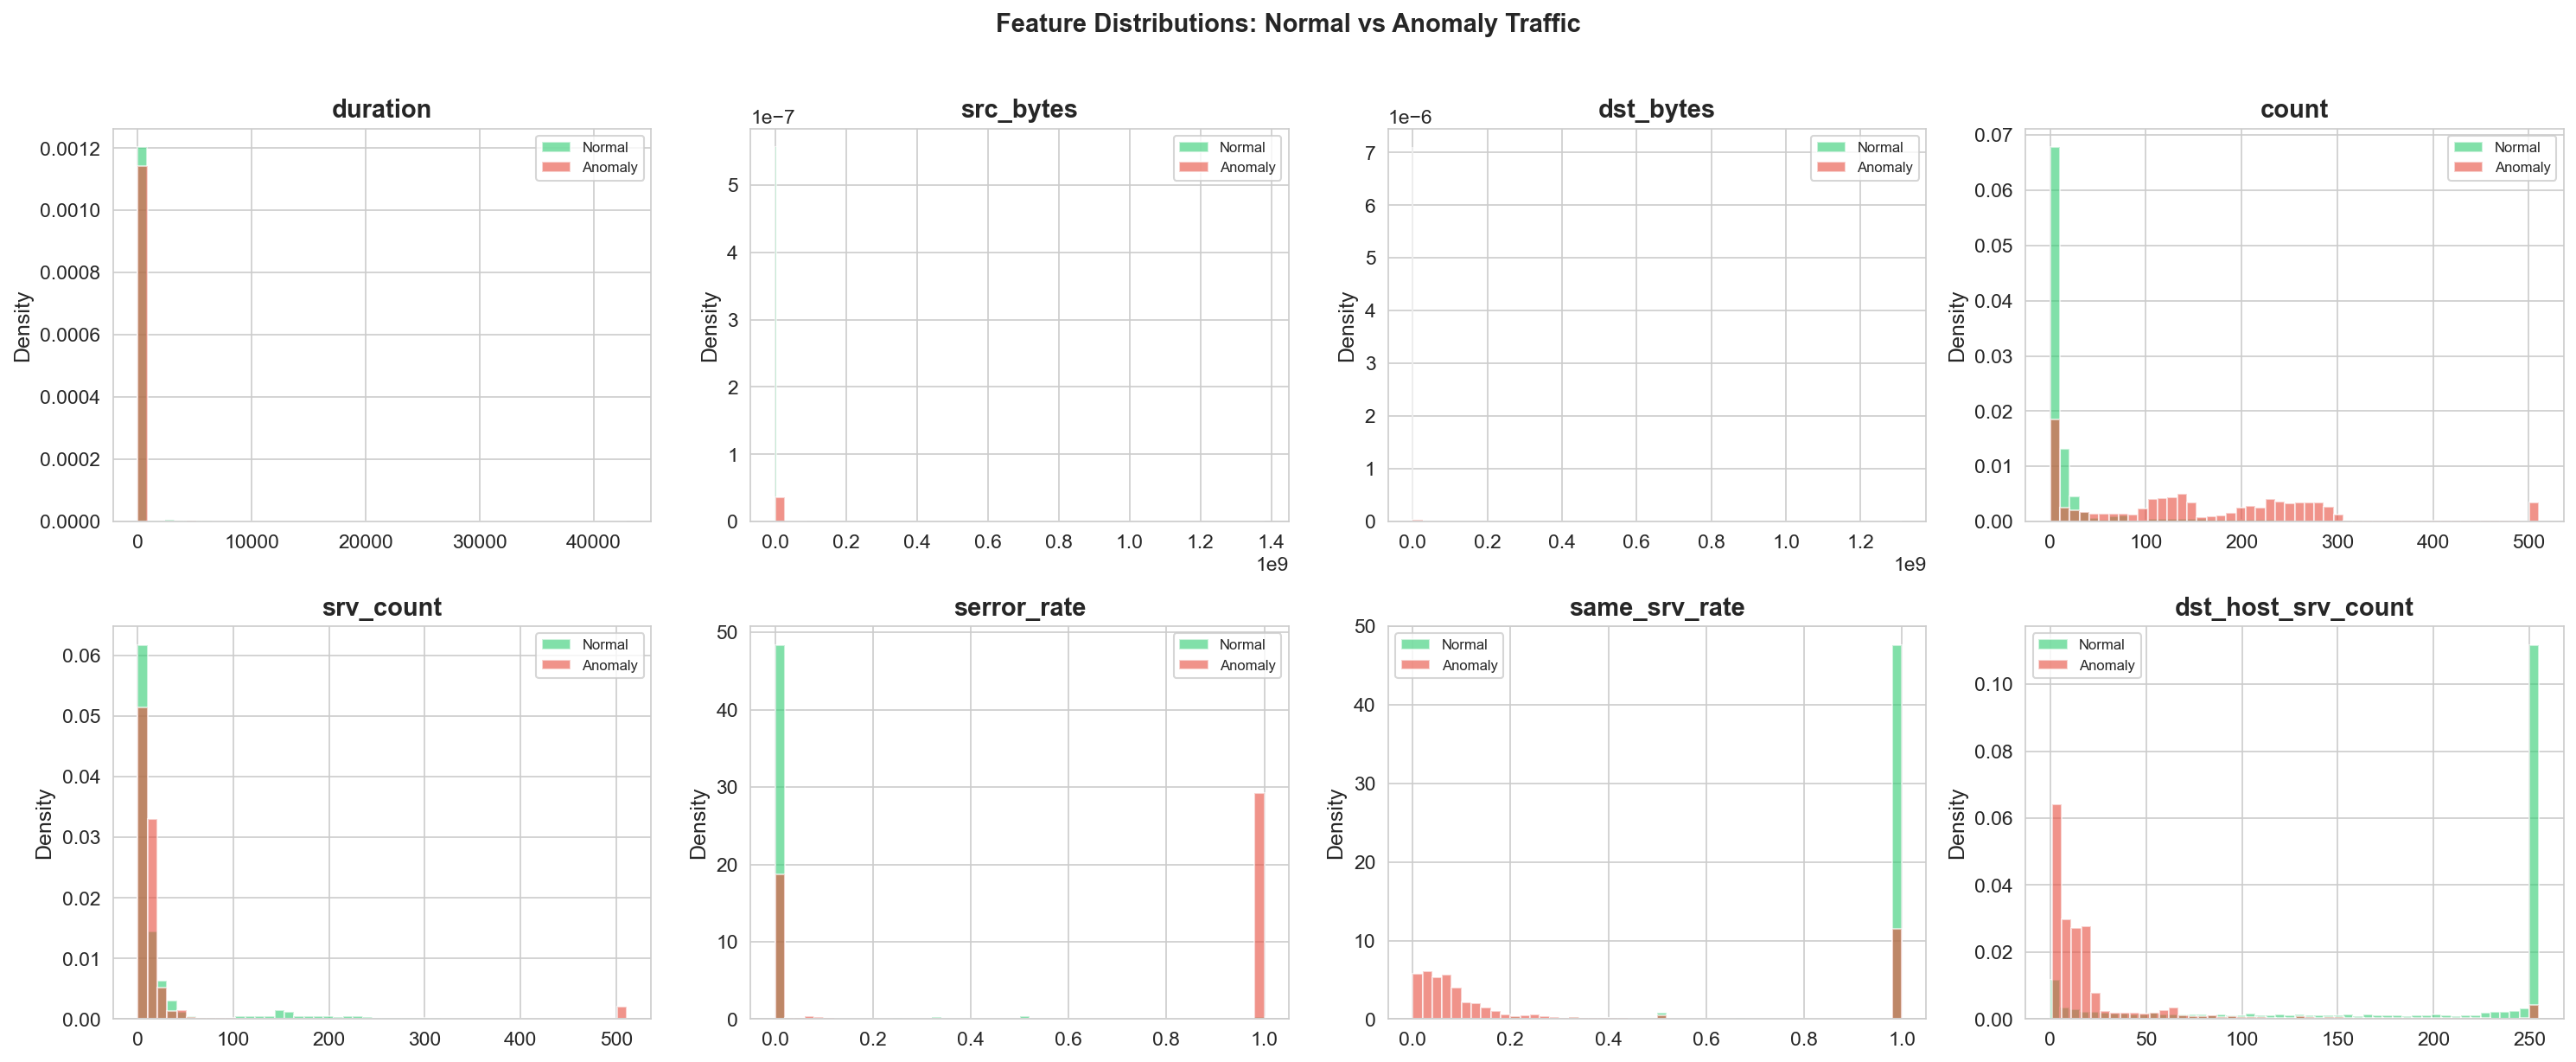
\includegraphics[width=\textwidth]{results/feature_distributions.png}
    \caption{Feature distributions for selected numerical features}
    \label{fig:feat_dist}
  \end{subfigure}

  \vspace{4pt}

  \begin{subfigure}[b]{0.48\textwidth}
    \centering
    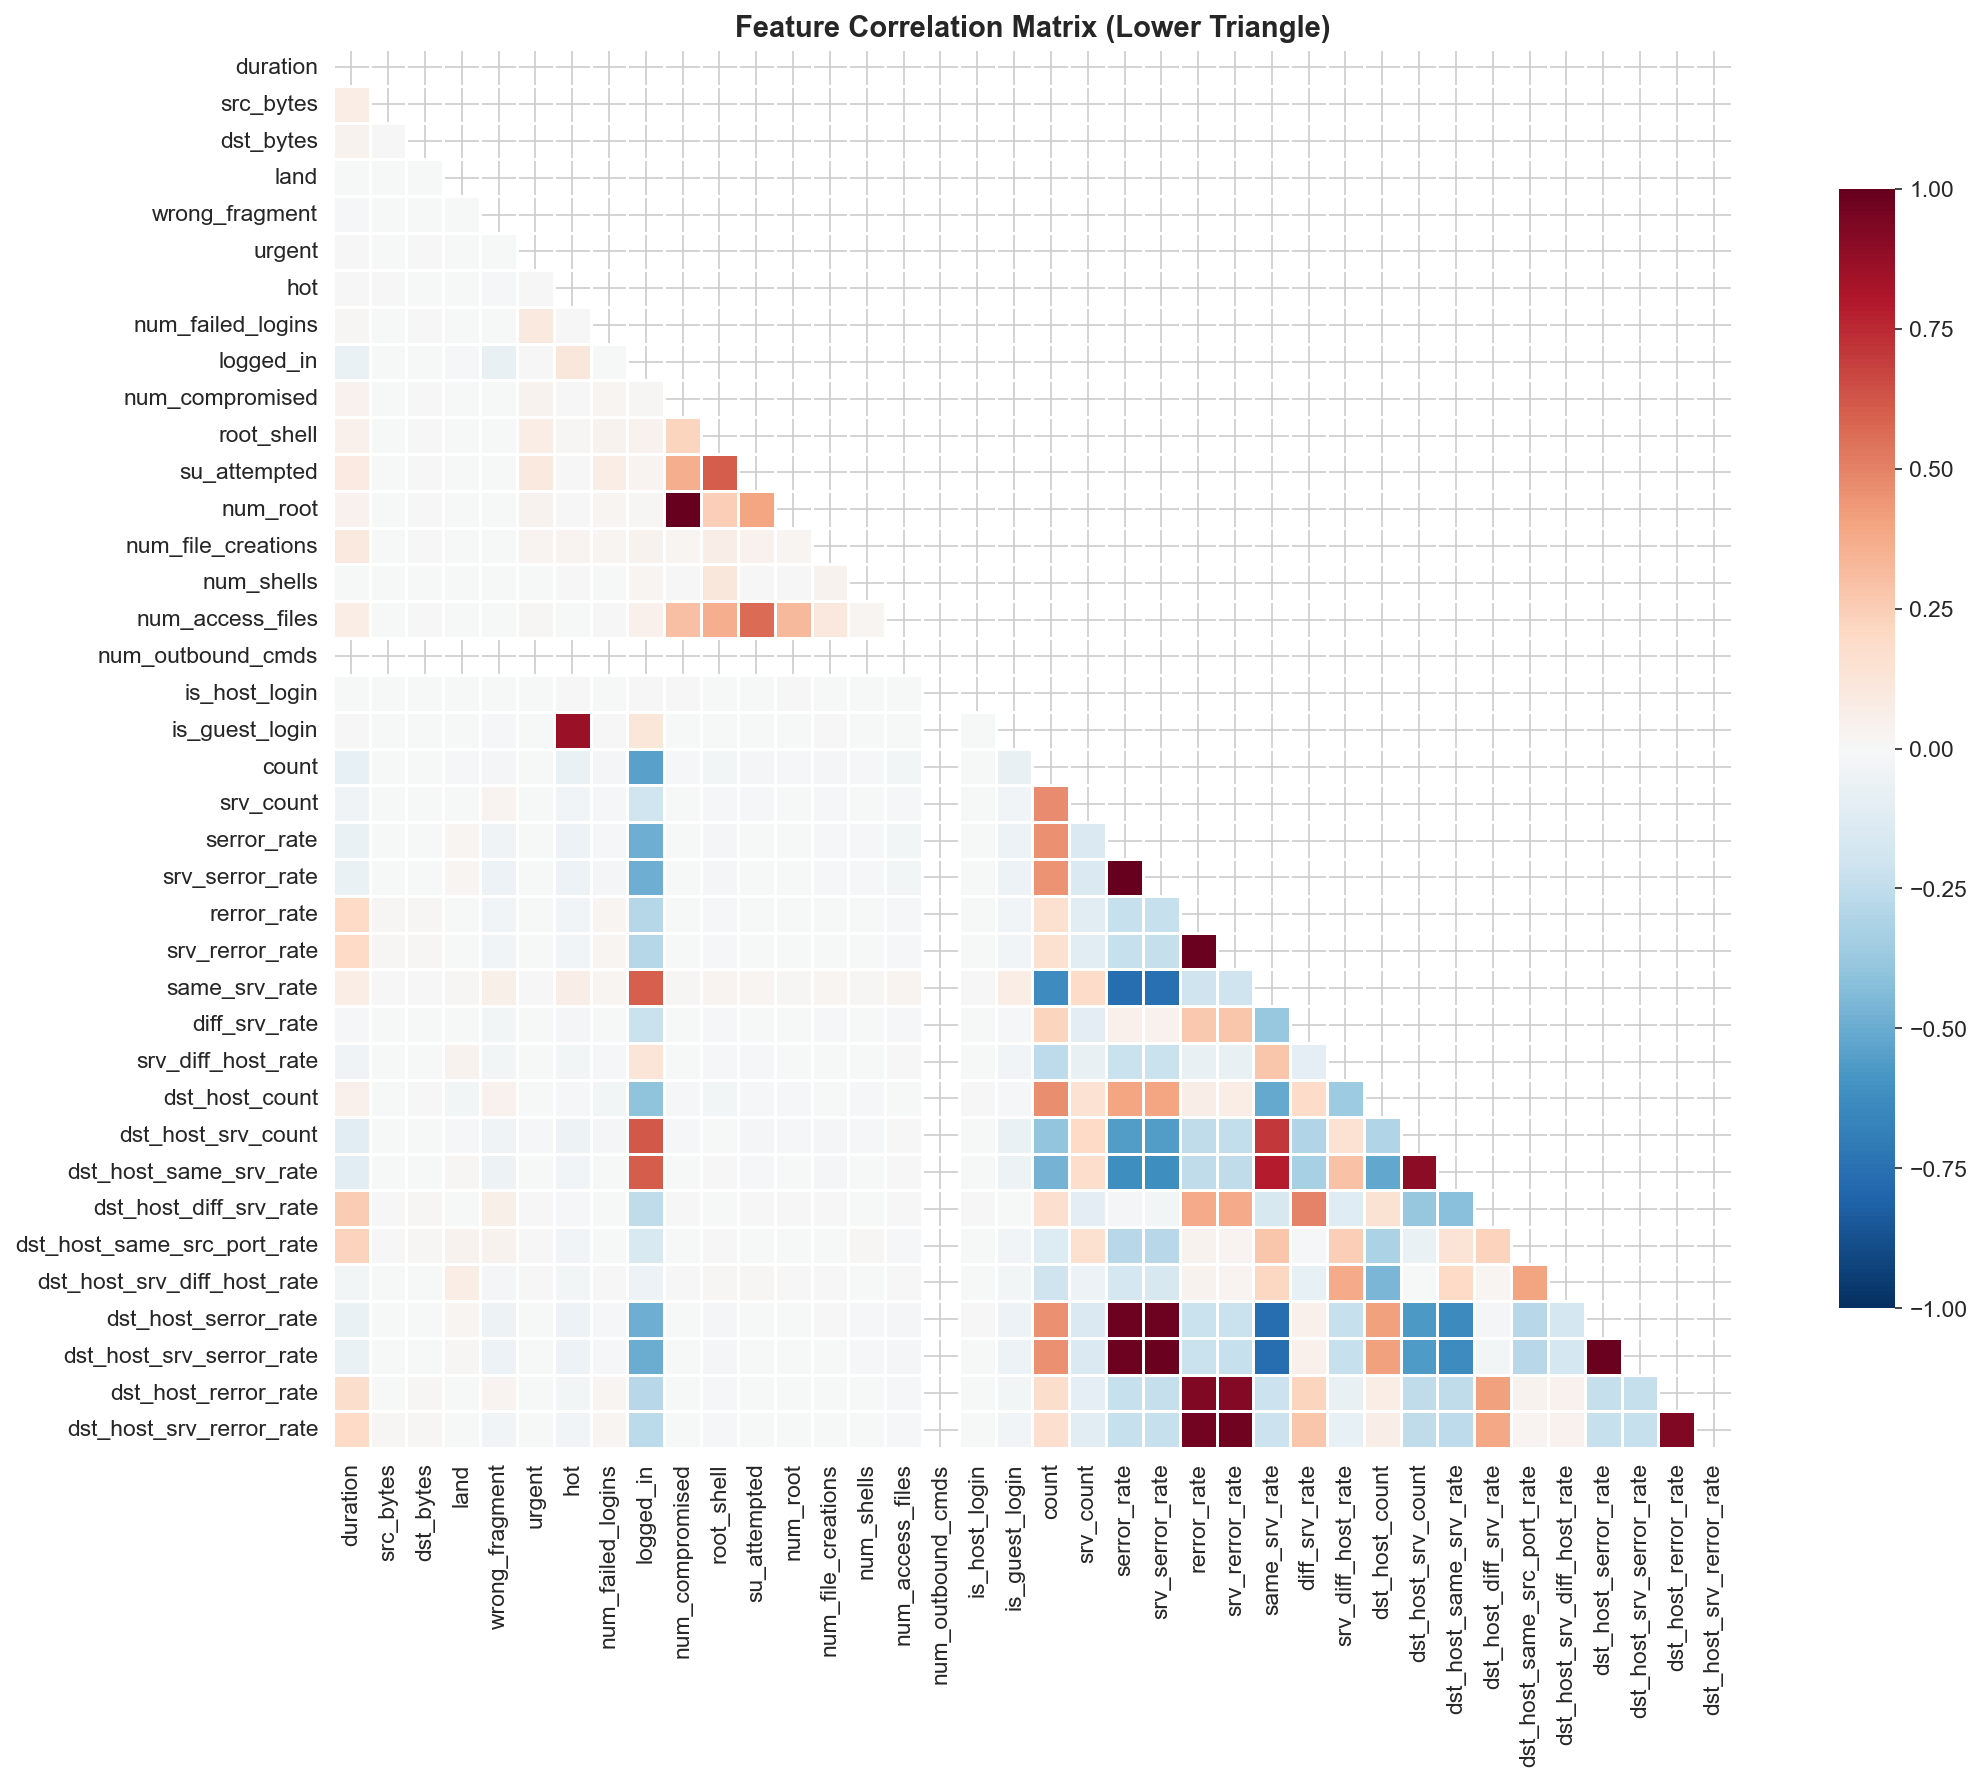
\includegraphics[width=\textwidth]{results/correlation_matrix.png}
    \caption{Feature correlation matrix (lower triangle)}
    \label{fig:corr_mat}
  \end{subfigure}
  \hfill
  \begin{subfigure}[b]{0.48\textwidth}
    \centering
    
\includegraphics[width=\textwidth]{results/dimensionality_reduction.png}
    \caption{PCA and t-SNE projections (Blue: Normal, Red: Attack)}
    \label{fig:dimred}
  \end{subfigure}

  \caption{EDA Overview: class distributions, feature distributions, correlation
  structure, and 2-D projections of 5,000 test-set samples via PCA and t-SNE.}
  \label{fig:eda_overview}
\end{figure*}

The projections confirm that normal and attack traffic form broadly separable---though
partially overlapping---clusters, justifying the anomaly-detection framing and
providing an upper-bound intuition for achievable performance.

\section{Preprocessing Pipeline}
\label{sec:preprocessing}

The preprocessing decisions are motivated directly by the EDA findings summarised
in Table~\ref{tab:preproc}.

\begin{table}[H]
  \centering
  \caption{Preprocessing Steps and Rationale}
  \label{tab:preproc}
  \begin{tabular}{p{2.8cm}p{5.0cm}}
    \toprule
    \textbf{Step} & \textbf{Rationale} \\
    \midrule
    Label Encoding         & Convert categorical features to integers; Z-Score requires numerical input; tree ensembles handle ordinal encoding natively. \\[3pt]
    Drop Zero-Variance     & \texttt{num\_outbound\_cmds} carries no information. \\[3pt]
    Feature Engineering    & Three new features capture domain-relevant interaction effects (see below). \\[3pt]
    Standard Scaling       & Fitted on \emph{normal training data only}; stabilises Z-Score scoring and improves Isolation Forest convergence. \\[3pt]
    Semi-Supervised Split  & Models trained on 67,343 normal records only; evaluated on 22,544 mixed test records. \\
    \bottomrule
  \end{tabular}
\end{table}

\subsection{Engineered Features}
Three domain-informed features are appended to the 40-dimensional post-selection
feature set, yielding a final $d=43$ feature vector.

\begin{enumerate}
  \item \textbf{Bytes Ratio}:
        \[
          f_1 = \frac{\texttt{src\_bytes}}{\texttt{dst\_bytes} + 1}
        \]
        Captures network flow asymmetry; large values indicate potential data
        exfiltration.

  \item \textbf{Error Rate Difference}:
        \[
          f_2 = \texttt{serror\_rate} - \texttt{srv\_serror\_rate}
        \]
        Flags inconsistency between connection- and service-level error rates,
        characteristic of scan traffic.

  \item \textbf{Service Diversity Ratio}:
        \[
          f_3 = \frac{\texttt{diff\_srv\_rate}}{\texttt{same\_srv\_rate} + \epsilon},
          \quad \epsilon = 10^{-6}
        \]
        Measures multi-service access patterns; elevated values indicate horizontal
        scan behaviour.
\end{enumerate}

\subsection{Semi-Supervised Data Preparation}
The \texttt{StandardScaler} is fitted \emph{exclusively} on the 67,343 normal
training records and applied to both training and test sets.  This simulates the
realistic operational constraint that the detector has access only to benign
traffic during calibration.

Post-scaling diagnostics confirm correctness:
\begin{itemize}
  \item Mean of scaled training data: $\approx 0.0$.
  \item Standard deviation of scaled training data: $\approx 0.988$.
\end{itemize}

\section{Methods}
\label{sec:methods}

\subsection{Z-Score Statistical Thresholding}
\label{ssec:zscore}

Let $\mathbf{x} \in \mathbb{R}^{d}$ denote a network connection feature vector.
On the normal training set $\mathcal{D}_n$ we compute:
\[
  \mu_j = \frac{1}{|\mathcal{D}_n|} \sum_{\mathbf{x} \in \mathcal{D}_n} x_j,
  \qquad
  \sigma_j = \sqrt{\frac{1}{|\mathcal{D}_n|} \sum_{\mathbf{x} \in \mathcal{D}_n}
             (x_j - \mu_j)^2},
\]
for each feature dimension $j \in \{1,\ldots,d\}$.

An observation is flagged as an anomaly if \emph{any} standardised feature value
exceeds a scalar threshold $\tau$:
\begin{equation}
  \hat{y}(\mathbf{x}) =
  \begin{cases}
    1 & \text{if } \max_j \left|\dfrac{x_j - \mu_j}{\sigma_j}\right| > \tau,\\[6pt]
    0 & \text{otherwise.}
  \end{cases}
\end{equation}

The threshold $\tau$ is tuned via grid search over $\tau \in \{1.0, 2.0, 3.0, 4.0, 5.0\}$
on the test set, maximising the F1-score.  The optimal value is $\tau^{*} = 2.0$.

\textbf{Key properties}:
\begin{itemize}
  \item Simple and interpretable---the analyst can directly inspect which features
        triggered the alarm.
  \item Assumes near-Gaussian feature distributions---partially violated here due
        to heavy-tailed byte-count features, but mitigated by standard scaling.
  \item Requires only means and standard deviations; $O(|\mathcal{D}_n| \cdot d)$
        training complexity.
\end{itemize}

\subsection{Isolation Forest}
\label{ssec:iforest}

Liu \emph{et al.}\ \cite{liu2008} formalise the intuition that anomalies are ``few
and different,'' hence are \emph{easy to isolate} via random partitioning.

An \emph{isolation tree} $T$ is constructed recursively:
\begin{enumerate}
  \item Select a feature $j$ uniformly at random from $\{1,\ldots,d\}$.
  \item Select a split point $s$ uniformly at random from
        $[\min_j(\mathbf{X}), \max_j(\mathbf{X})]$.
  \item Partition $\mathbf{X}$ into left and right subsets; recurse.
\end{enumerate}

Given an ensemble of $T$ trees, the anomaly score for observation $\mathbf{x}$ is:
\begin{equation}
  s(\mathbf{x}, n) = 2^{-\frac{\mathbb{E}[h(\mathbf{x})]}{c(n)}},
\end{equation}
where $h(\mathbf{x})$ is the path length (number of splits) to isolate $\mathbf{x}$,
and $c(n) = 2 \ln(n-1) - \frac{2(n-1)}{n}$ is the expected path length in a random
binary search tree of $n$ nodes.  Observations with $s \approx 1$ are anomalous;
$s \approx 0.5$ indicates normality.

\textbf{Hyperparameter tuning}: The \emph{contamination} parameter $\rho$
(expected fraction of anomalies in the data) is swept over $\{0.01, 0.05, 0.1, 0.2, 0.3, 0.4, 0.5\}$;
the value $\rho^{*} = 0.1$ optimises the F1-score.  The number of trees is fixed at
$T=100$ and the sub-sampling size at 256.

\textbf{Key properties}:
\begin{itemize}
  \item Scale-invariant: does not rely on feature distributions.
  \item Sub-linear training complexity relative to dataset size due to sub-sampling.
  \item Robust to high dimensionality through random feature selection.
\end{itemize}

\section{Experimental Results}
\label{sec:results}

\subsection{Evaluation Protocol}
Both models are evaluated on the 22,544-sample test set using:
\begin{itemize}
  \item \textbf{Accuracy} --- $\frac{\text{TP}+\text{TN}}{N}$.
  \item \textbf{Precision} --- $\frac{\text{TP}}{\text{TP}+\text{FP}}$.
  \item \textbf{Recall} --- $\frac{\text{TP}}{\text{TP}+\text{FN}}$.
  \item \textbf{F1-Score} --- Harmonic mean of Precision and Recall.
  \item \textbf{ROC-AUC} --- Area under the Receiver Operating Characteristic curve.
\end{itemize}

Anomaly~($y=1$) is the \emph{positive} class; normal traffic~($y=0$) is negative.

\subsection{Hyperparameter Sensitivity}

Fig.~\ref{fig:hparam} shows the sensitivity of both detectors to their respective
key hyperparameters.

\begin{figure*}[ht]
  \centering
  \begin{subfigure}[b]{0.48\textwidth}
    \centering
    
\includegraphics[width=\textwidth]{results/zscore_threshold_tuning.png}
    \caption{Z-Score: threshold $\tau$ sensitivity.  $\tau=2$ gives best F1/AUC.}
    \label{fig:zscore_tune}
  \end{subfigure}
  \hfill
  \begin{subfigure}[b]{0.48\textwidth}
    \centering
    
\includegraphics[width=\textwidth]{results/if_contamination_tuning.png}
    \caption{Isolation Forest: contamination $\rho$ sensitivity.  $\rho=0.1$ is optimal.}
    \label{fig:if_tune}
  \end{subfigure}
  \caption{Hyperparameter sensitivity: Z-Score threshold (left) and Isolation Forest
  contamination (right).  Both sweeps are evaluated on the test set by F1-score.}
  \label{fig:hparam}
\end{figure*}

\subsection{Confusion Matrices and ROC Curves}

Fig.~\ref{fig:results_overview} presents the complete evaluation panel: confusion
matrices for both models side by side, and the ROC comparison spanning the full width.

\begin{figure*}[ht]
  \centering
  \begin{subfigure}[b]{0.48\textwidth}
    \centering
    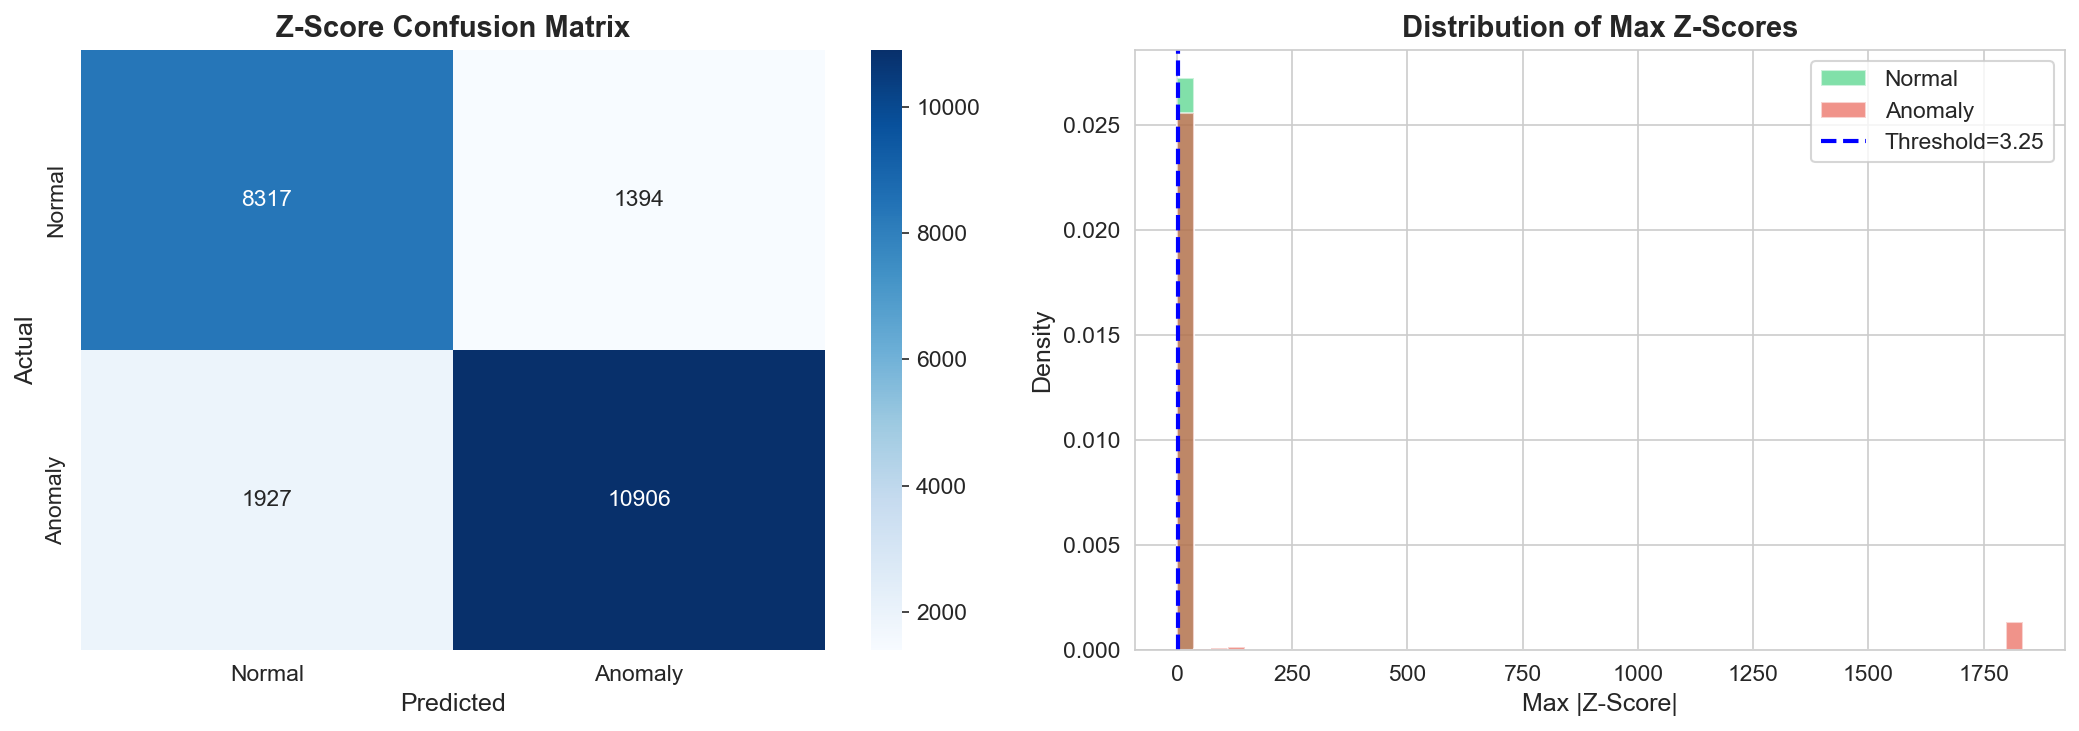
\includegraphics[width=\textwidth]{results/zscore_results.png}
    \caption{Z-Score Thresholding confusion matrix}
    \label{fig:zscore_cm}
  \end{subfigure}
  \hfill
  \begin{subfigure}[b]{0.48\textwidth}
    \centering
    
\includegraphics[width=\textwidth]{results/isolation_forest_results.png}
    \caption{Isolation Forest confusion matrix}
    \label{fig:if_cm}
  \end{subfigure}

  \vspace{4pt}

  \begin{subfigure}[b]{0.80\textwidth}
    \centering
    
\includegraphics[width=\textwidth]{results/roc_comparison.png}
    \caption{ROC curves: Isolation Forest (AUC = 0.939) dominates Z-Score (AUC = 0.899)}
    \label{fig:roc}
  \end{subfigure}

  \caption{Results overview: confusion matrices on the NSL-KDD test set (top) and
  ROC comparison (bottom).  Isolation Forest achieves higher AUC at all operating
  points, while Z-Score offers superior precision.}
  \label{fig:results_overview}
\end{figure*}

\subsection{Summary Performance Metrics}
Table~\ref{tab:results} reports the key metrics for both models.

\begin{table}[H]
  \centering
  \caption{Baseline Model Performance on NSL-KDD Test Set}
  \label{tab:results}
  \begin{tabular}{lccccc}
    \toprule
    \textbf{Model}         & \textbf{Acc.} & \textbf{Prec.} & \textbf{Rec.} & \textbf{F1} & \textbf{AUC} \\
    \midrule
    Z-Score ($\tau=2$)      & 85.27\%       & 88.67\%        & 84.98\%       & 86.79\%     & 89.93\%      \\
    Isolation Forest ($\rho=0.1$)
                            & 84.86\%       & 86.04\%        & 87.63\%       & 86.82\%     & 93.91\%      \\
    \bottomrule
  \end{tabular}
\end{table}

\subsection{Discussion}
\label{ssec:discussion}

Both models achieve F1-scores above 86\% in the binary anomaly-detection task,
confirming that the feature space contains sufficient discriminative signal and
that the preprocessing pipeline is effective.

Key observations:
\begin{enumerate}
  \item \textbf{Precision vs.\ Recall trade-off}: Z-Score exhibits higher precision
        (88.67\% vs.\ 86.04\%) while Isolation Forest achieves higher recall (87.63\%
        vs.\ 84.98\%).  In operational IDS deployments, the preferred operating point
        depends on the relative cost of False Negatives (missed attacks) versus False
        Positives (analyst alert fatigue).

  \item \textbf{AUC advantage of Isolation Forest}: The 4-point AUC gap (93.91\%
        vs.\ 89.93\%) is substantial and traces to Isolation Forest's non-parametric,
        non-linear decision boundary.  The Z-Score model is constrained by its
        per-feature, max-statistic aggregation, which discards feature correlations
        and joint distributional structure.

  \item \textbf{Dimensionality reduction insight}: The t-SNE visualisation
        (Section~\ref{ssec:dimred}) reveals that some attack clusters are tightly
        packed and well-separated from normal traffic, while others partially overlap.
        This distribution motivates the use of non-linear, ensemble-based, and deep
        models in subsequent phases.

  \item \textbf{Feature engineering impact}: The three engineered features
        ($f_1$: bytes asymmetry, $f_2$: error-rate inconsistency, $f_3$: service
        diversity) encode domain knowledge not directly present in the raw features.
        They are expected to be particularly informative for Probe and R2L categories.

  \item \textbf{Limitations}: Both detectors are trained without access to
        attack-type labels during learning.  As a result, they lack the fine-grained
        supervision needed to distinguish between attack categories---a capability
        important for incident response.  Deep anomaly models (autoencoders, VAEs) and
        sequence models (LSTMs) are planned for Phase~2.
\end{enumerate}

\section{Conclusion}
\label{sec:conclusion}

This paper presents a semi-supervised anomaly detection framework for network
intrusion detection on the NSL-KDD dataset.  Motivated by the fundamental
limitation of signature-based IDS---their inability to detect zero-day attacks---we
adopted a one-class learning paradigm that trains exclusively on benign traffic.

A rigorous Exploratory Data Analysis guided the design of a principled preprocessing
pipeline.  Two complementary baseline detectors were implemented and evaluated:

\begin{itemize}
  \item \textbf{Z-Score Thresholding} (Accuracy~85.27\%, AUC~89.93\%): a simple,
        interpretable parametric detector that provides a transparent performance floor.
  \item \textbf{Isolation Forest} (Accuracy~84.86\%, AUC~93.91\%): a non-parametric,
        tree-based ensemble that achieves superior discriminative power, particularly
        at low false-positive rates.
\end{itemize}

These baselines establish a rigorous evaluation framework for Phase~2, which will
explore deep anomaly detectors---autoencoders, variational autoencoders, and
LSTM-based sequence models---capable of exploiting non-linear feature interactions
and temporal traffic dynamics.

\begin{thebibliography}{9}

\bibitem{chandola2009}
V. Chandola, A. Banerjee, and V. Kumar,
``Anomaly detection: A survey,''
\textit{ACM Computing Surveys}, vol.~41, no.~3, pp.~1--58, 2009.

\bibitem{denning1987}
D. E. Denning,
``An intrusion-detection model,''
\textit{IEEE Transactions on Software Engineering},
vol.~SE-13, no.~2, pp.~222--232, Feb. 1987.

\bibitem{liu2008}
F. T. Liu, K. M. Ting, and Z.-H. Zhou,
``Isolation forest,''
in \textit{Proc.\ 8th IEEE Int.\ Conf.\ Data Mining (ICDM)},
pp.~413--422, 2008.

\bibitem{roesch1999}
M. Roesch,
``Snort: Lightweight intrusion detection for networks,''
in \textit{Proc.\ 13th USENIX Systems Administration Conf.\ (LISA)},
pp.~229--238, 1999.

\bibitem{sakurada2014}
M. Sakurada and T. Yairi,
``Anomaly detection using autoencoders with nonlinear dimensionality
reduction,''
in \textit{Proc.\ MLSDA 2nd Workshop Mach.\ Learn.\ Sensory Data Anal.},
pp.~4--11, 2014.

\bibitem{scholkopf2001}
B. Sch\"{o}lkopf, J. C. Platt, J. Shawe-Taylor, A. J. Smola, and R. C. Williamson,
``Estimating the support of a high-dimensional distribution,''
\textit{Neural Computation}, vol.~13, no.~7, pp.~1443--1471, Jul. 2001.

\bibitem{tavallaee2009}
M. Tavallaee, E. Bagheri, W. Lu, and A. A. Ghorbani,
``A detailed analysis of the KDD CUP 99 data set,''
in \textit{Proc.\ 2nd IEEE Symp.\ Comput.\ Intell.\ Security Defense Appl.\
(CISDA)}, pp.~1--6, 2009.

\end{thebibliography}

\end{document}
